\chapter{From White Paper to Research Plan}
\label{chap:e28}

\begin{chapteropening}
By now the whole book's toolbox is full: complex amplitude and phase (Chapter \ref{chap:e01}), bandwidth and coherence time (Chapter \ref{chap:e02}), Poisson and shot noise (Chapter \ref{chap:e03}), second-order coherence \(g^{(2)}\) and the Siegert relation (Chapter \ref{chap:e08}), intensity interferometry and the van Cittert--Zernike theorem (Chapter \ref{chap:e10}), from visibility to imaging (Chapter \ref{chap:e11}), quantum estimation and SPADE (Chapter \ref{chap:e12}), event tables and clocks (Chapter \ref{chap:e13}), correlators (Chapter \ref{chap:e14}), error budgets and feasibility (Chapter \ref{chap:e15}), on to treating stars, compact stars, black holes, and transients as quantum light sources (Chapters \ref{chap:e17}--\ref{chap:e20}) and the first-generation science cases (Chapter \ref{chap:e25}). The tools are ready, but what this chapter answers is a question not so ``physical'' yet decisive of whether anything can happen at all: \textbf{how do you turn a beautiful idea into a research plan that can really be executed, and can really fail?} We walk through a clear path: \textbf{pose the science question \(\to\) select target and method \(\to\) write the error budget and estimate achievable precision \(\to\) plan the instrument and data pipeline \(\to\) lay out milestones and register risks \(\to\) write the plan}, and at each step map some formula from an earlier chapter onto an item in the proposal that can be reviewed, reproduced, and scored. The tone of this chapter turns slightly toward ``your'' next action: after reading it, you should be able to rewrite an idea into work packages, acceptance metrics, and failure criteria.
\end{chapteropening}

\section{Start from the science question: pick the right target before talking about instruments}
\label{sec:e28-question}

The most common failure in writing a plan is not ``the instrument is not good enough'' but \textbf{getting the order backward from the start}: first falling in love with an instrument or a fashionable word (``quantum,'' ``entanglement,'' ``network''), then going to look for a topic. The correct order is always: first ask a \textbf{science question} that can be observationally falsified, then ask which \textbf{observable} can answer it, and only last ask what instrument, what precision, and what kind of target source are needed.

An executable science question usually looks like this: not ``I want to study stars'' but ``just how much dimmer is the equator than the poles of this rapid rotator, and how flattened is it''; not ``I want to do quantum astronomy'' but ``are the photon statistics of this natural-laser candidate line thermal or coherent?'' The former is vague and cannot converge; the latter immediately points to an observable (the variation of \(|V|^2\) with position angle, the deviation of \(g^{(2)}(0)\) from 1) and immediately points to a set of instrument requirements.

When selecting targets, the three yardsticks of Chapter \ref{chap:e25} still apply: \textbf{brightness} decides ``whether there are photons,'' \textbf{angular scale} decides ``whether these photons can become parameters,'' and \textbf{external prior} decides ``whether the parameters can be uniquely translated into physics.'' But in writing a plan one must add one more yardstick, often overlooked in pure science discussion yet a lifeline in a proposal: \textbf{whether there is still a product after failure}. A good plan, even if the main target is not detected, should leave behind something reusable: a well-calibrated event-table format, a released version of the correlator, a calibration-star table, a set of time-synchronized null tests. Write this into target selection and you will not stake everything on a single detection that may fall through.

The product of this step is plain but is the foundation of the whole plan: a one-sentence science question + one definite observable + one ``why this target and not that'' ranking rationale. All the subsequent error budgets, instrument design, and milestones serve this one sentence. Many of the common misconceptions listed in Chapter \ref{chap:e27} (mistaking multimode thermal light for a laser, mistaking single-direction baselines for being able to determine shape, mistaking the visibility for something whose phase can be read directly) stem from \textbf{cutting corners at this step}: rushing to the instrument before thinking through ``what to measure, what can be falsified.''

\section{What can be landed in the near term: making intensity interferometry a routine data product}
\label{sec:e28-nearterm}

First the tier that \textbf{can be done now}. In the near term (the foreseeable next few years), the most mature and the most deserving of top priority for a proposal is turning the intensity interferometry already repeatedly validated by VERITAS and MAGIC from ``a single demonstration'' into ``a reproducible data product'' \citep{2020NatAs...4.1164A,2024MNRAS.529.4387A}. The quantum-network telescope is fascinating, but it belongs to a later stage (Chapter \ref{chap:e24}) and should not occupy the first batch of work packages in the near term.

The main observables of this stage are: the second-order coherence \(\hat g^{(2)}_{ab}(\tau)\), the squared visibility \(|V_{ab}|^2\), each telescope's target photon rate, the zero-baseline contrast, the background dilution factor, and the covariance on each baseline. The question is: how do we judge whether a near-term project is \textbf{actually mature}? Statements like ``the detector is available'' and ``the telescope is big enough'' cannot go into a proposal, because they cannot be accepted. We need a scorable readiness criterion.

Write the project readiness as a \textbf{ratio vector}, each entry being ``actual capability \(\div\) requirement'':
\begin{equation}
  \bm{r}=
  \left(
  \frac{R_\gamma}{R_{\rm req}},\;
  \frac{\sigma_{t,{\rm req}}}{\sigma_t},\;
  \frac{\beta_0}{\beta_{\rm req}},\;
  \frac{\sigma_{{\rm sys,req}}}{\sigma_{\rm sys}},\;
  \frac{N_{\rm cal}}{N_{{\rm cal,req}}}
  \right).
  \label{eq:e28-readiness}
\end{equation}
\begin{formulaexplain}
\(\bm r\) is the project readiness vector. Each entry is ``actual capability over requirement'': photon rate, timing precision, zero-baseline contrast, systematic-error floor, calibration sample. Only when all five entries are \textbf{simultaneously} \(\ge1\) does the near-term project close. Any entry \(<1\) is a shortfall that must be filled first.
\end{formulaexplain}
Accounting for each symbol, unit, and dimension clearly is the key to turning \eqref{eq:e28-readiness} from a ``pretty vector'' into a ``reconcilable checklist.'' \(R_\gamma\) is each telescope's effective target photon rate, units \(\mathrm{s^{-1}}\), set jointly by the collecting area, quantum efficiency, filter bandwidth, and target brightness; \(R_{\rm req}\) is the photon rate needed to reach the target precision. \(\sigma_t\) is the relative time-synchronization error between telescopes, often in ps or ns; note this entry is \textbf{requirement over capability} (\(\sigma_{t,{\rm req}}/\sigma_t\)), because the smaller the error the better, so the ``requirement'' goes in the numerator. \(\beta_0\) is the zero-baseline correlation contrast (dimensionless), measuring how much correlation signal the instrument can recover when ``two telescopes look at the same beam''; \(\beta_{\rm req}\) is the required contrast. \(\sigma_{\rm sys}\) is the residual systematic-error floor after calibration (dimensionless, same units as \(|V|^2\)), likewise entered as ``requirement over capability.'' \(N_{\rm cal}\) is the number of usable calibration stars or calibration observations, and \(N_{\rm cal,req}\) is the number required.

The value of this vector is that it \textbf{prevents a single entry from masking a shortfall}. Take a counterexample: suppose your photon rate is extremely high, \(R_\gamma/R_{\rm req}=5\), looking very abundant; but if the systematic-error floor \(\sigma_{\rm sys}=3\times10^{-5}\) is larger than the small \(|V|^2\) signal you want to measure, then \(\sigma_{\rm sys,req}/\sigma_{\rm sys}<1\), and the project is still immature: no amount of photons can flatten a systematic bias. Research on intensity-interferometry arrays stresses this repeatedly: baseline length, \(u,v\) coverage, background control, and zero-baseline calibration must all close \textbf{together}, none can be missing \citep{2006ApJ...649..399L,2013APh....43..331D,2022MNRAS.512.1722K}.

\begin{figure}[tbp]
\centering
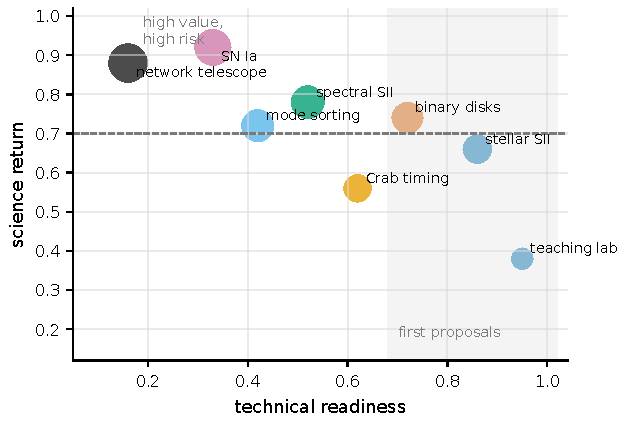
\includegraphics[width=0.86\linewidth]{figures/generated/chapter_22/ch22_roadmap_trade_space.pdf}
\caption{Technical maturity, science return, cost, and risk in the roadmap. The horizontal axis is technical maturity, the vertical axis is science return, and the larger the point, the greater the cost pressure. Tasks in the upper right with high maturity are suited to be written as near-term proposals; tasks in the upper left with high scientific value but needing a pathfinder first belong to the mid-to-far term. This figure is the visualization of the ``look at the shortfall before talking value'' approach of Eq.\ \eqref{eq:e28-readiness}.}
\label{fig:e28-trade-space}
\end{figure}

When writing a near-term plan, the more concrete the topic the better. Executable topics can be ``measure the angular diameters of 10--30 bright stars near 416 nm with four IACTs, and release the correlator and calibration library,'' or ``use the same pipeline to compare the \(|V|^2\) models of binaries, Be-star disks, and rapid rotators.'' Each paper should release: the event-table format description, the correlator version number, the time-shift null test, the calibration-star table, the baseline geometry, and the posterior samples. This way, even if some targets are not detected, reusable instrument knowledge is left behind, exactly the ``product after failure'' of the previous section.

\section{Error budget and feasibility: first estimate the precision you can reach}
\label{sec:e28-budget}

The item most indispensable in a plan, and the first thing a referee looks at, is the \textbf{error budget}: the core tool of Chapter \ref{chap:e15}. It answers two questions: ``How accurately can this observation ultimately measure the observable?'' ``Is it statistical noise, or some systematic error, that limits this precision?'' A proposal without an error budget is like saying ``I want to do it, but I don't know how well I can do it,'' and is almost certain to be rejected.

The skeleton of an error budget is to \textbf{add in quadrature} the various independent errors. Why add in quadrature rather than directly? Because for several \textbf{mutually independent} random errors, the total variance equals the sum of the individual variances (a direct consequence of the additivity of variances of independent random variables in probability theory, covered in Chapter \ref{chap:e03}). Let the standard deviations of the error sources be \(\sigma_{\rm stat},\sigma_{\rm cal},\sigma_{\rm bg},\sigma_{\rm model},\sigma_{\rm sel}\); then the total error is
\begin{equation}
  \sigma_{\rm tot}^2
  =
  \sigma_{\rm stat}^2
  +\sigma_{\rm cal}^2
  +\sigma_{\rm bg}^2
  +\sigma_{\rm model}^2
  +\sigma_{\rm sel}^2 .
  \label{eq:e28-error-budget}
\end{equation}
\begin{formulaexplain}
Each term is the standard deviation of one error source's contribution to the final observable (same dimensions as the observable): \(\sigma_{\rm stat}\) statistical, \(\sigma_{\rm cal}\) calibration, \(\sigma_{\rm bg}\) background, \(\sigma_{\rm model}\) model, \(\sigma_{\rm sel}\) selection effect. Independent errors add in variance, so \textbf{the largest term dominates the total error}: go press that one down first.
\end{formulaexplain}
Grounding each term, and also explaining where each comes from. \(\sigma_{\rm stat}\) is statistical noise, from the finite sample of Poisson or correlated counts, falling as \(T^{-1/2}\) with integration time. \(\sigma_{\rm cal}\) is calibration error, from imperfections in zero-baseline contrast, time synchronization, and polarization and spectral response. \(\sigma_{\rm bg}\) is background, from night-sky light, continuum, or companion-star blending. \(\sigma_{\rm model}\) is model error, from the stellar disk, supernova photosphere, BLR, or maser geometry you use to fit being itself insufficiently realistic. \(\sigma_{\rm sel}\) is selection effect, from biases introduced by triggering, weather, and target selection. The practical reading of Eq.\ \eqref{eq:e28-error-budget} is: \textbf{adding in quadrature means the largest term has a veto}: if one term is three times larger than the rest, the others after square-rooting barely change the total, and all your effort should go to cutting that one term. Statistical tools like MCMC, nested sampling, or posterior predictive checks can help you compute \(\sigma_{\rm stat}\) and the parameter posterior accurately, but they \textbf{cannot substitute for} the physical error terms \(\sigma_{\rm cal}\), \(\sigma_{\rm model}\) themselves \citep{2013PASP..125..306F,2009MNRAS.398.1601F,1979ApJ...228..939C,2013ApJ...764..167S}.

The term one should estimate first in the error budget is often the statistical term \(\sigma_{\rm stat}\), because it directly tells you ``whether this target is doable at all.'' The intensity-interferometry signal-to-noise given in Chapter \ref{chap:e15} is a known result that can be used by name (Hanbury Brown's classic expression):
\begin{equation}
  \left(\frac{S}{N}\right)
  =
  A\,\alpha\,n\,|V|^2
  \sqrt{\frac{\Delta f\,T}{2}} .
  \label{eq:e28-snr}
\end{equation}
\begin{formulaexplain}
The signal-to-noise of intensity interferometry: \(A\) collecting area, \(\alpha\) quantum efficiency, \(n\) the spectral photon flux per unit area per unit bandwidth (spectral flux density), \(|V|^2\) the squared-visibility signal, \(\Delta f\) the electronic bandwidth, \(T\) the integration time. The crux is that the signal-to-noise grows only as \(\sqrt{T}\): to double the precision, the integration time must quadruple.
\end{formulaexplain}
Laying out the units of the symbols: \(A\) has units \(\mathrm{cm^2}\), \(\alpha\) is dimensionless (typically \(0.2\text{--}0.3\)), \(n\) has units \(\mathrm{cm^{-2}\,Hz^{-1}\,s^{-1}}\) (also understandable as the photon occupation per mode per second \(\bar n_\nu\) times a geometric factor, see Chapter \ref{chap:e15}), \(\Delta f\) has units Hz, and \(T\) has units s. Hidden in this equation are three intuitions that must be internalized when writing a plan: first, the signal is \(|V|^2\) rather than \(|V|\): once the target is partially resolved and \(|V|^2\) drops, the signal-to-noise loses \textbf{by the square}, which is why the angular scale must match the baseline. Second, the signal-to-noise grows only as \(\sqrt{\Delta f\,T}\): raising the precision to double costs four times the observing time or four times the electronic bandwidth, and this \(\sqrt{\cdot}\) law directly sets your requested duration. Third, \(n\) depends on wavelength and bandwidth, and the appeal of spectral multiplexing is precisely that it can accumulate this SNR in parallel across many channels (next section).

Plug in a set of real numbers to land the feasibility. Take a pair of \(100\,\mathrm{m^2}\) telescopes (i.e.\ \(A=10^6\,\mathrm{cm^2}\)), quantum efficiency \(\alpha=0.25\), electronic bandwidth \(\Delta f=200\,\mathrm{MHz}=2\times10^8\,\mathrm{Hz}\), integration time \(T=5\,\mathrm{h}=1.8\times10^4\,\mathrm{s}\). Here the order of magnitude most easily misestimated is the dimensionless combination \(A\alpha n\): substituting \(A=10^6\,\mathrm{cm^2}\), \(\alpha=0.25\), and a spectral photon flux of about \(n\sim4\times10^{-11}\,\mathrm{cm^{-2}\,Hz^{-1}\,s^{-1}}\) for an \(m_V\simeq6\) hot star in a narrow band, we get \(A\alpha n\sim10^{-5}\). Note in particular that this number is \textbf{far less than 1}: it is in fact the degeneracy parameter of thermal light, that is, the order of magnitude of the photon occupation per mode per second \(\bar n_\nu\) times a geometric factor; precisely because the \(\bar n_\nu\ll1\) of a visible-light thermal star, the intensity-interferometry signal is so weak and so hard to obtain (which is also why one must scrape it together with large area and long integration). Take the signal on a representative baseline where the source is partially resolved, \(|V|^2\sim0.5\) (at the true zero baseline \(|V|^2\to1\); here we have already left the zero baseline by some amount and the source is partially resolved). Then \(\sqrt{\Delta f\,T/2}=\sqrt{2\times10^8\times1.8\times10^4/2}=\sqrt{1.8\times10^{12}}\approx1.3\times10^6\), so \(S/N\sim10^{-5}\times0.5\times1.3\times10^6\approx6.7\), that is, of order a few sigma, consistent with the estimate of LeBohec and Holder that ``a several-sigma detection of an \(m_V\simeq6.7\) source can be made within 5 hours'' for the present generation of instruments \citep{2006ApJ...649..399L,2013APh....43..331D}. Conversely, if the target is 1 magnitude fainter, the photon flux \(n\) drops to about \(40\%\), and in the same time the signal-to-noise drops to about \(40\%\); to make it back one must raise \(T\) to about \(6\) times; such numbers must be written into the feasibility subsection of the proposal, not vaguely stated as ``we believe it can be done.''

\section{Instrument and data pipeline: from event table to public archive}
\label{sec:e28-pipeline}

Having estimated the precision, one must next answer ``what instrument and what data pipeline will realize this precision.'' This section pushes the plan from ``how accurately can it be measured'' to ``how to measure it, what the data look like, and how others reproduce it.''

The data product of a near-term project is still simple: one blue-filter \(|V|^2\) plus the covariance of a few baselines. But a far-sighted plan should plan how the \textbf{data product will grow}. The mid-term goal is to expand ``single-channel \(|V|^2\)'' into a \textbf{multi-channel event table}: spectrally resolved intensity interferometry can compare the angular scales inside and outside spectral lines (the disk is larger than the photosphere, and the \(|V|^2\) of the line region falls faster); polarization-resolved correlation can examine the magnetic-field geometry, scattering, and strong-field radiation; picosecond-level event tables can treat the photon statistics themselves as a new time-domain data product. The appeal of spectral multiplexing is that each spectral channel has a longer coherence time, and multiple channels can accumulate the signal-to-noise of Eq.\ \eqref{eq:e28-snr} in parallel; the price is that the data rate, inter-channel calibration, and dispersion model all become more complex \citep{2021sf2a.conf..335L,2022MNRAS.512.1722K,2024MNRAS.529.4387A}.

Writing the data product of the multi-channel stage as a set is when the plan enters engineering language:
\begin{equation}
  \bm{d}=
  \left\{
  H_{ab}^{\nu p}(\tau),\;
  \widehat{|V_{ab}^{\nu p}|^2},\;
  C_{\nu_i\nu_j}^{p_i p_j},\;
  \bm{\Sigma}
  \right\}.
  \label{eq:e28-data}
\end{equation}
\begin{formulaexplain}
\(\bm d\) is the complete data product of the multi-channel stage, not just \(|V|^2\): \(H_{ab}^{\nu p}(\tau)\) is the delay histogram, \(\widehat{|V_{ab}^{\nu p}|^2}\) is the calibrated squared visibility, \(C_{\nu_i\nu_j}^{p_i p_j}\) is the cross-frequency/cross-polarization covariance, and \(\bm\Sigma\) is the covariance matrix binding these quantities together. \textbf{How the data are stored, normalized, and released} determines whether the project has reached the engineering stage.
\end{formulaexplain}
Explaining the meaning and role of each term. \(H_{ab}^{\nu p}(\tau)\) is the coincidence-count histogram at telescope pair \(a,b\), frequency channel \(\nu\), polarization channel \(p\), and delay \(\tau\): it is the raw product the correlator (Chapter \ref{chap:e14}) directly spits out, and \(\hat g^{(2)}\) is its normalized shape. \(\widehat{|V_{ab}^{\nu p}|^2}\) is the spatial-coherence observable calibrated from the histogram (the van Cittert--Zernike bridge of Chapter \ref{chap:e10} connects it to the source's angular structure). \(C_{\nu_i\nu_j}^{p_i p_j}\) is the covariance between different frequency or polarization channels, carrying the ``genuinely new'' physics of the angular-scale contrast inside versus outside spectral lines and between different polarizations. \(\bm\Sigma\) is the covariance matrix of the whole dataset, which must be used when fitting object parameters, rather than pretending the points are independent. Writing merely one sentence ``we will do multi-channel quantum observation'' is far from enough; writing clearly the storage format, normalization convention, and release method of each quantity in \(\bm d\) is an engineering-grade plan.

\begin{figure}[tbp]
\centering
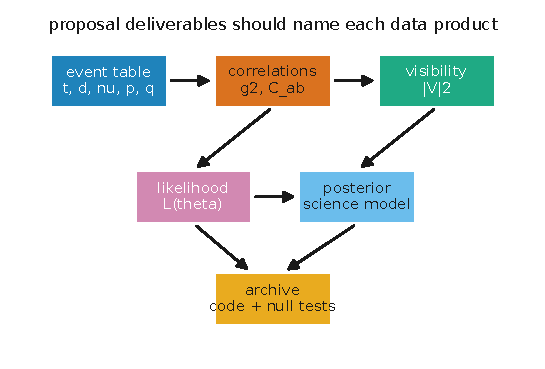
\includegraphics[width=0.88\linewidth]{figures/generated/chapter_22/ch22_data_product_stack.pdf}
\caption{The product chain from proposal to public data. The event table retains each photon's arrival time, telescope, frequency, polarization, and quality flag; the correlator turns it into \(g^{(2)}\) and covariance; the spatial model gives \(|V|^2\); the likelihood and posterior connect it to object parameters; and the archive layer must include the code, version numbers, and null tests. Each quantity in Eq.\ \eqref{eq:e28-data} corresponds to one link in this chain.}
\label{fig:e28-data-products}
\end{figure}

When planning the data pipeline, there is a principle running through the whole book worth writing on the plan's first page: \textbf{the event table is the common language}. Whether it is a classroom tabletop HBT demonstration (Chapter \ref{chap:e26}), a small-aperture pathfinder, or a large-facility observation, they can all share the same ``arrival time + telescope + frequency + polarization + quality flag'' event-table format and the same version of correlator \citep{2016SPIE.9907E..0NZ,2025MNRAS.537.2527M}. This means the data format you define in the plan lets teaching, pathfinder, and main facility connect seamlessly, which is itself a design that lowers risk and raises reproducibility.

\section{Risks and milestones: let the plan fail, but fail with value}
\label{sec:e28-risk}

A plan that writes only ``what we will do and what we expect to see'' is in fact not yet ready to face reality. In reality the target will be fainter than expected, the systematic error will stick at some floor, and the transient will trigger too late. A mature plan must proactively write out \textbf{milestones} (breaking success into acceptable nodes) and a \textbf{risk register} (listing where things may go wrong together with mitigation plans).

First the milestones. An executable milestone must \textbf{simultaneously} specify ``what to measure'' and ``what counts as success,'' otherwise it is only a vision. Write it as a quintuple:
\begin{equation}
  m_j=
  \left(
  O_j,\;
  \sigma_{O,j}^{\rm goal},\;
  T_j,\;
  N_{{\rm null},j},\;
  D_{{\rm release},j}
  \right).
  \label{eq:e28-milestone}
\end{equation}
\begin{formulaexplain}
\(m_j\) is the \(j\)-th milestone: \(O_j\) is the observable to be measured, \(\sigma_{O,j}^{\rm goal}\) is the target precision to be reached, \(T_j\) is the completion date or observing time needed, \(N_{{\rm null},j}\) is the number of null tests that must be passed, and \(D_{{\rm release},j}\) is the data product to be released. A milestone that \textbf{simultaneously pins down} observable, precision, time, verification, and delivery keeps the roadmap from stalling at slogans.
\end{formulaexplain}
Grounding each term and giving typical values. \(O_j\) is the observable, for example \(g^{(2)}(0)-1\), \(|V|^2\), the angular-scale ratio inside versus outside a line, or the distance \(D_A\). \(\sigma_{O,j}^{\rm goal}\) is the target precision, coming directly from the error budget \eqref{eq:e28-error-budget} of the previous section: a milestone's precision goal cannot be pulled out of thin air but must be a number the error budget computes. \(T_j\) is the completion date or the machine time required. \(N_{{\rm null},j}\) is the number of null tests: a near-term project can require \(N_{\rm null}\ge2\) (time-shift and off-source); a mid-term multi-channel project should rise to \(N_{\rm null}\ge4\) (adding off-band, wrong-polarization, injection-recovery); and a far-term network project must further include independent acceptance of link fidelity and storage decoherence. \(D_{{\rm release},j}\) is the delivered data product, for example some subset of Eq.\ \eqref{eq:e28-data} plus the code and version numbers. Writing all five items lets a review judge, item by item, which node has passed and which still owes.

\begin{figure}[tbp]
\centering
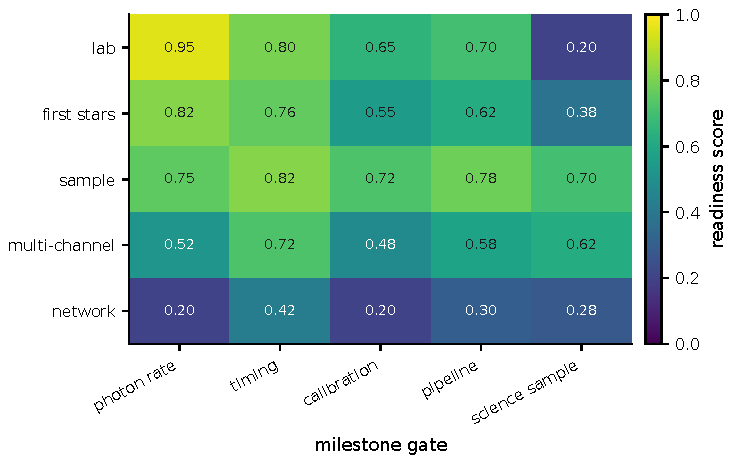
\includegraphics[width=0.90\linewidth]{figures/generated/chapter_22/ch22_milestone_gates.pdf}
\caption{The milestone-gate matrix for different stages. Course experiments and first-generation stellar intensity interferometry are already fairly mature in photon rate, timing, and pipeline, but multi-channel calibration and the network stage still have clear gaps. The numbers in the figure are only \emph{examples} of the readiness scores a proposal should explicitly quantify, used to illustrate how each item of Eq.\ \eqref{eq:e28-milestone} should be scored, and do not represent any facility commitment.}
\label{fig:e28-gates}
\end{figure}

Now the risks. The essence of a risk register is to bind each risk to a \textbf{failure criterion}: not only saying ``what may go wrong'' but also ``at what degree one should change the plan, and change it to what.'' Several concrete examples, all quantifiable by the earlier formulas: if the target star is 1 mag fainter than expected, then by Eq.\ \eqref{eq:e28-snr} the photon flux drops and the signal-to-noise falls to about \(40\%\): the mitigation is to prepare brighter backup targets in advance or extend the machine time. If the systematic-error floor stalls at \(\sigma_{\rm sys}\sim3\times10^{-5}\), then by Eq.\ \eqref{eq:e28-error-budget} many small \(|V|^2\) signals are drowned by this term: the mitigation is to build a calibration-star library first to press \(\sigma_{\rm cal}\) down. If a Type Ia trigger is 10 days late, the shell is larger but the luminosity has already fallen and the model uncertainty \(\sigma_{\rm model}\) rises: the mitigation is to write the trigger response as a hard metric and set a clear abandonment criterion for late-arriving events. If the quantum-network link gives only very few high-fidelity entangled pairs per day, the science mode should \textbf{fall back} to local mode sorting or ordinary intensity interferometry, rather than forcing the network scheme (Chapter \ref{chap:e24}).

\begin{figure}[tbp]
\centering
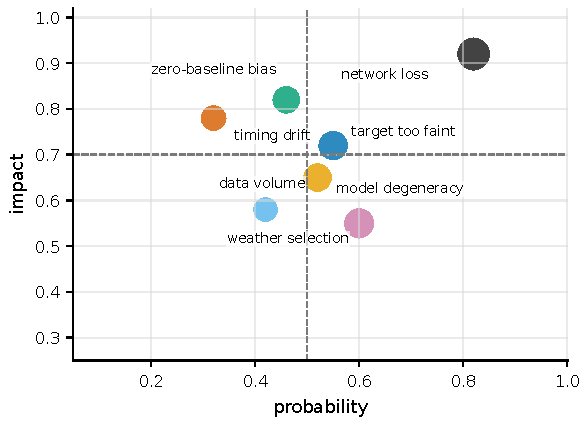
\includegraphics[width=0.86\linewidth]{figures/generated/chapter_22/ch22_risk_register.pdf}
\caption{The roadmap's risk-register figure. The horizontal and vertical axes are occurrence probability and impact, and the larger the point, the weaker the existing mitigation. Risks in the upper-right corner must have mitigations in place before the project begins: network loss needs a short-baseline pathfinder first, zero-baseline bias needs a calibration-star library first, and an over-faint target needs preset clear trigger and abandonment criteria.}
\label{fig:e28-risk}
\end{figure}

These two things together convey perhaps the most important attitude of this chapter: \textbf{a good research plan allows itself to fail, but makes every failure tell the next stage what to change}. A night with zero detections, as long as it leaves behind a well-calibrated event table, passed null tests, and a released version of the correlator, has advanced the instrument knowledge one step, far better than a plan that ``reports only successes.''

\section{Weaving the whole book into a path: from course project to research topic}
\label{sec:e28-path}

Finally, twist the six preceding steps into one rope, and see how it grows from a classroom exercise all the way into a submittable research plan, and where along this path far-term ideas like the quantum network should be placed.

The starting point can be very small. The course project (Chapter \ref{chap:e26}) begins with tabletop HBT, event-table simulation, uniform-disk fitting, the Fisher information of SPADE (Chapter \ref{chap:e12}), and false-alarm calculation: these exercises look like toys, yet they already walk a miniature version of the path ``pose the question \(\to\) design the observation \(\to\) estimate the precision \(\to\) write the plan.'' One level up, a smaller research topic is well suited to revolve around \textbf{one pipeline}: time synchronization, correlator, calibration library, target sample, or an open-data notebook: each can stand as its own paper and each leaves behind a reusable product. Higher still, a fuller science topic can aim at the line angular scale of a Be-star \(\mathrm{H}\alpha\) disk, the multi-baseline model of a rapid rotator, the phase-resolved photon statistics of the Crab pulsar, the systematic errors of a Type Ia distance toy model, or a joint experiment of local mode sorting (Chapter \ref{chap:e12}) with adaptive optics. At the top level, a large collaboration then connects these topics to CTAO/IACT, ELT/VLTI/CHARA, Rubin, SKA, gravitational-wave networks, and even quantum-network laboratories.

Regarding the \textbf{far term}: when the quantum-network telescope becomes the main line, the plan must honestly stratify. Many information-theoretic benefits do not require a complete quantum network: local mode sorting and phase-sensitive measurement (Chapter \ref{chap:e12}) can already improve the information efficiency of small-separation and brightness-moment estimation, and this can be advanced \textbf{now} \citep{2016PhRvX...6c1033T,2017PhRvL.118g0801T}. Two-photon astrometry, single-photon-assisted or linear-optics pathfinders aim to stably couple astronomical light with laboratory quantum resources, and belong to the mid-term \citep{2023PhRvL.130p0801M,2024SPIE13095E..1NR}. True entanglement-assisted long-baseline interferometry requires the entanglement-distribution rate, quantum storage time, frequency-conversion efficiency, Bell fidelity, and astronomical synchronization to meet their targets \textbf{simultaneously}, and belongs to a later stage \citep{2025PhRvA.111d3701M,2026PhRvA.113a2608P}. This resource threshold has already been written in Chapter \ref{chap:e24} as constraints on link rate, storage time, and effective fidelity; in writing a plan one need only remember one order of magnitude: at baseline \(B=1000\,\mathrm{km}\) the light-travel time is \(B/c\simeq3.3\,\mathrm{ms}\), and a ground-based km-scale baseline needs only \(\mu\mathrm{s}\)-to-ms-level synchronization, but a global or space baseline rapidly amplifies the storage and distribution pressure. If any one of link loss, storage decoherence, or useful photon rate fails to meet its target, the network scheme is not yet sufficient to replace ordinary intensity interferometry, and at that point an honest plan should fall back to the tier that can be done in the near term, rather than overdrawing the future in the proposal.

\begin{figure}[tbp]
\centering
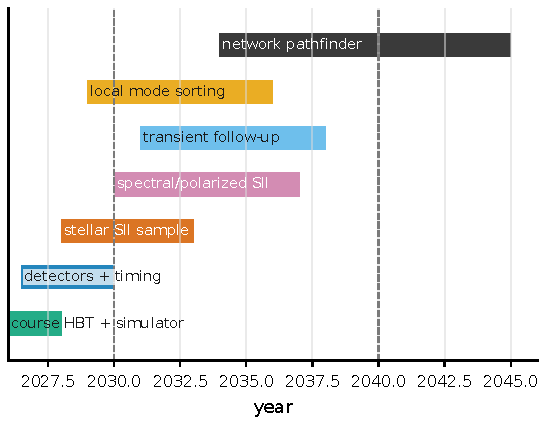
\includegraphics[width=0.92\linewidth]{figures/generated/chapter_22/ch22_program_timeline.pdf}
\caption{The staged timeline from course HBT to quantum-network pathfinder. Early tasks build talent, event tables, timing, and calibration; mid-term tasks produce the first-generation science sample and multi-channel correlation; far-term tasks should be written as facility-level roadmaps only after local mode sorting, link, and storage metrics meet their targets. This timeline is precisely the path of this chapter, ``growing from a course project into a research topic.''}
\label{fig:e28-timeline}
\end{figure}

Compress all of this into one operational acceptance standard: \textbf{a qualified research plan must at minimum list the new observables, the event-table fields, the data-estimation steps, the units and typical ranges of each symbol, two or more null tests, and the data, code, or instrument constraints that will remain even after failure}. Meet these, and your plan can be reproduced, reviewed, and improved; otherwise the word ``quantum'' stays only in the title, landing on no falsifiable number. This is precisely the last thing the whole book wants to teach you: turn tools into questions, turn questions into observations, and turn observations into a plan that others can carry forward.

\section*{Chapter Summary}
\addcontentsline{toc}{section}{Chapter Summary}

\begin{itemize}
  \item \textbf{The order cannot be reversed.} First pose the science question, then fix the observable, and only last talk about instruments and precision. Beyond brightness, angular scale, and external prior, target selection must ask one more thing: ``Is there still a product after failure?''
  \item \textbf{Maturity must be acceptable.} Use the ratio vector \eqref{eq:e28-readiness} to score a near-term project: photon rate, timing, zero-baseline contrast, systematic error, and calibration sample must \textbf{simultaneously} meet their targets, and any entry \(<1\) is a shortfall that must be filled first.
  \item \textbf{The error budget is the foundation.} Independent errors add in variance (Eq.\ \eqref{eq:e28-error-budget}), and the largest term has a veto; statistical noise can be estimated by Eq.\ \eqref{eq:e28-snr}, the signal-to-noise grows only as \(\sqrt{\Delta f\,T}\), doubling the precision costs quadruple machine time, and this must be written into the feasibility subsection (Chapter \ref{chap:e15}).
  \item \textbf{The data pipeline must be engineered.} Write the data product as a set \eqref{eq:e28-data}: delay histogram, \(|V|^2\), cross-channel covariance, and full covariance matrix; define the format well so that teaching, pathfinder, and main facility can share the same event table (Chapters \ref{chap:e13}, \ref{chap:e14}).
  \item \textbf{Milestones and risks are written together.} The milestone quintuple \eqref{eq:e28-milestone} simultaneously pins down observable, precision, time, number of null tests, and delivery; risks must be written together with failure criteria, letting the plan fail, but fail in a way that tells the next stage what to change.
  \item \textbf{The far term must be honestly stratified.} Local mode sorting can be done now, the pathfinder is mid-term, and the entanglement-assisted network is the main line only when several metrics meet their targets simultaneously (Chapter \ref{chap:e24}); if they do not, honestly fall back to the tier that can be done in the near term.
\end{itemize}

\medskip
\noindent\textbf{Questions to Ponder}
\begin{itemize}
  \item You hold a readiness vector \eqref{eq:e28-readiness} in which the photon-rate entry is \(R_\gamma/R_{\rm req}=4\) and the other four entries are all around \(0.9\). Should this project be written as a proposal now? If not, into which entry would you first invest machine time and funds?
  \item Use Eq.\ \eqref{eq:e28-snr} to estimate: if the electronic bandwidth \(\Delta f\) is raised from \(200\,\mathrm{MHz}\) to \(800\,\mathrm{MHz}\), with all else unchanged, to roughly what fraction of the original is the integration time needed to reach the same signal-to-noise shortened?
  \item Pick a science case from Chapter \ref{chap:e25} for yourself, and try to write it as a milestone quintuple \eqref{eq:e28-milestone}: what should its \(O_j\), \(\sigma_{O,j}^{\rm goal}\), \(N_{{\rm null},j}\), and \(D_{{\rm release},j}\) be filled with? Which item can you not yet answer, and what step does that tell you the plan still lacks?
\end{itemize}
